\documentclass{sig-alternate}

%Nice code listings
\usepackage{minted}
\usepackage[hidelinks]{hyperref}
\usepackage{url}
\newcommand{\code}[1]{\texttt{#1}}
\newcommand{\floor}[1]{\left\lfloor #1 \right\rfloor}
\begin{document}
%
% --- Author Metadata here ---
\conferenceinfo{HPTCDL}{'14 New Orleans, Louisiana USA}
%\CopyrightYear{2007} % Allows default copyright year (20XX) to be over-ridden - IF NEED BE.
%\crdata{0-12345-67-8/90/01}  % Allows default copyright data (0-89791-88-6/97/05) to be over-ridden - IF NEED BE.
% --- End of Author Metadata ---

\title{Operator polymorphism for distributed computing in Julia}

\numberofauthors{2}

\author{
% 1st. author
\alignauthor
Jiahao Chen\\
       \affaddr{Massachusetts Institute of Technology}\\
       \affaddr{Computer Science and Artificial Intelligence Laboratory}\\
       \affaddr{77 Massachusetts Avenue}\\
       \affaddr{Cambridge, Massachusetts 02139, USA}\\
       \email{jiahao@mit.edu}\\
% 2nd. author
\alignauthor
Alan Edelman\\
       \affaddr{Massachusetts Institute of Technology}\\
       \affaddr{Department of Mathematics and Computer Science and Artificial Intelligence Laboratory}\\
       \affaddr{77 Massachusetts Avenue}\\
       \affaddr{Cambridge, Massachusetts 02139, USA}\\
       \email{edelman@mit.edu}
}

\date{15 October 2014}

\maketitle
\begin{abstract}
High level languages provide nice abstractions for most computing tasks, but fall short of providing useful abstractions for parallel computing.

The lack of useful abstractions poses significant challenges for users of parallel computing.

In this paper we study a primitive parallel algorithm, namely that of prefix reduction, and show how it can be implemented with operator overloading so that the parallelism occurs at the operational level, not the algorithmic level.

The ability to write such code shows that Julia's abstractions are useful for reasoning about the structure of parallel algorithms by successfully abstracting away implementation details.

Code reuse for other tasks as well like visualization.

\end{abstract}

\category{D.1.3}{Concurrent programming}{Distributed programming}
\category{D.3.2}{Programming languages}{Very high-level languages}
\category{G.1.0}{General numerical analysis}{Parallel algorithms}

\terms{Algorithms}

\keywords{Julia, prefix sum, scan}

\section{Introduction}
Nobody really understands how to do parallel computing. In practice, a lot of parallel computing code is mucky and gross because you have to embed all sorts of low level MPI initialization and communication primitives in your code.

How do the GPU Gems chapter showcase parallel prefix?

Can we do better to abstract away the low level communication protocols of a distributed algorithm?

In Julia we expose how overloading at the operator level parallelism can be used to showcase the essentials of what is going on while relegating the parallelism to a lower more primitive level. In other words, successful abstraction!

\section{The Julia language}

Julia is a very high level dynamic language designed specifically for technical computing~\cite{Bezanson2012}.

Type system and multiple dispatch. The type system is a resource for programmers, not just a low level compiler system that is hidden from the user. Being able to use types in user written code has turned out to be a great boon for writing technical code.

Polymorphism. Julia provides two distinct kinds of polymorphism. One is the paradigm of multimethods and the other is parametric polymorphism. We will focus more on how multimethods are helpful.

\section{The prefix reduction algorithm}

What is prefix reduction~\cite{Iverson1962,Ladner1980,Brent1982}? Making use of associativity (or approximate associativity side node about floating point and how it doesn't really matter for most applications)  to regroup operations to provide different execution strategies.

Parallel scan is one of the ur-algorithms for parallel computing~\cite{Kruskal1985,Blelloch1989,Bell2012}.
There are many applications for the basic prefix sum algorithm~\cite{Blelloch1990,Blelloch1993}, but to just name a few relevant for technical computing, we can do 

- stream compaction~\cite{Harris2007}

- parallel sort~\cite{Blelloch1989}

- polynomial interpolation~\cite{Egecioglu1990}

- list operations~\cite{Hillis1986,Gorlatch1999}

- solving linear systems of equations involving block tridiagonal matrices~\cite{Mathias1995}

- minimal coverings of black-and-white images~\cite{Moitra1991}

- string matching problems~\cite{Chi1992}

- random number generation~\cite{Lu1996}

- simulating finite state machines~\cite{Ladner1980}

The obvious thing to do is a serial reduction. Here is a left-associative version, \code{scanl!} (as it were), that computes partial sums in a left-associative fashion:

\begin{minted}{julia}
function scanl!(y, +)
    @inbounds for i=2:length(y)
        y[i] = y[i-1] + y[i]
    end
    y
end
\end{minted}

Here is a code listing for the special case of 8

\begin{minted}{julia}
function prefix8!(y, .+)
    length(y)==8 || error("length 8 only")
    for i in [2,4,6,8] y[i] = y[i-1] .+ y[i] end
    for i in [  4,  8] y[i] = y[i-2] .+ y[i] end
    for i in [      8] y[i] = y[i-4] .+ y[i] end
    for i in [    6  ] y[i] = y[i-2] .+ y[i] end
    for i in [ 3,5,7 ] y[i] = y[i-1] .+ y[i] end
    y
end
\end{minted}

It's nice that we can use infix notation

It's nice that the operator is passed as an argument the function. This means that we have just written a higher order function (or functional).

Here is a figure of the code rendered in Compose, a Julia package for declarative vector graphics~\cite{Compose.jl}. 

Here is a picture showing what happens

\begin{figure}
  \centering

  \mint{julia}|render(prefix_serial!(AccessArray(8),+))|
  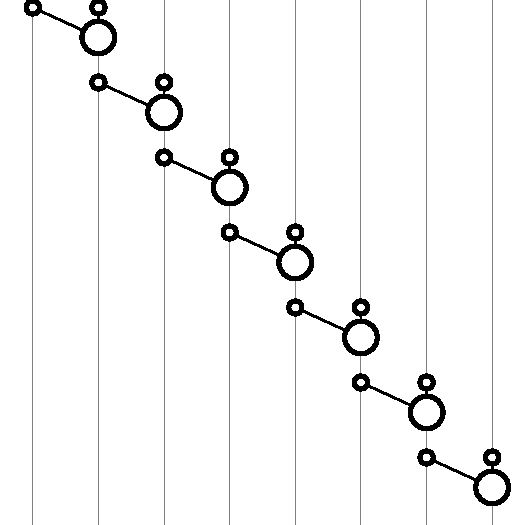
\includegraphics{serial}
  \vspace{12 pt}
  \mint{julia}|render(prefix8!(AccessArray(8),+))|
  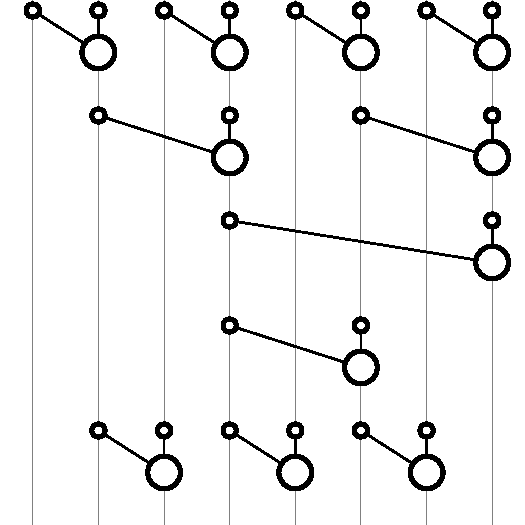
\includegraphics{tree}
  \caption{Above: operation order for the left-associative algorithm \code{scanl!}.
           Below: operation order for the tree algorithm \code{prefix8!}.
           The code listing for the \code{render} function is given in Section~\ref{sec:render}.}
  \label{fig:gates}
\end{figure}

Here is the tree branching version in the general case

\begin{minted}{julia}
function prefix!(y, .+)
    l=length(y)
    k=iceil(log2(l))
    #The "reduce" tree
    @inbounds for j=1:k, i=2^j:2^j:min(l, 2^k)
        y[i] = y[i-2^(j-1)] .+ y[i]
    end
    #The "broadcast" tree
    @inbounds for j=(k-1):-1:1, i=3*2^(j-1):2^j:
            min(l, 2^k)
        y[i] = y[i-2^(j-1)] .+ y[i]
    end
    y
end
\end{minted}

This is the classic algorithm of Brent and Kung~\cite{Brent1982}.

This is all serial code and all we have done is to do more work. So far. The point is that this algorithm is parallelizable as we shall see in the next section.

\section{Distributed computing using prefix reduction}

In this section we show how the prefix algorithm we wrote above can be run in a distributed computing context without modification. The key is to make use of overloading using the multimethod dispatch feature of Julia.

\subsection{Distributed computing in Julia}

\subsection{Parallel prefix}

\begin{minted}{julia}
#Add a specified number of processors
addprocs(max(0, Sys.CPU_CORES-nprocs()))

@show nprocs() #Current number of processes
@show procs()  #List of processes by index

import Base: fetch, length
fetch(t::Vector) = map(fetch, t) #Vectorize fetch

#Define elementary operations on remote data
length(r1::RemoteRef)=length(fetch(r1))
+(r1::RemoteRef,r2::RemoteRef)=
    @spawnat r2.where fetch(r1)+fetch(r2)
*(r1::RemoteRef,r2::RemoteRef)=
    @spawnat r2.where fetch(r1)*fetch(r2)
\end{minted}

It is straightforward to show from the definition of \code{prefix!} that the first tree on $p$ processors has depth $\floor{\log_2 p}$ and the second tree has depth $1 + \floor{\log_2 \frac p 3}$. Since the serial code \code{scanl!} has depth $p-1$, the theoretical speedup ratio, ignoring communication overhead, is therefore

\begin{equation}
    r (p) = \frac {p-1} {\floor{\log_2 p} + 1 + \floor{\log_2 \frac p 3}}.
    \label{eq:scaling-theory}
\end{equation}

Here is a figure summarizing benchmark timings for a sample problem. We generate $p$ square random matrices with Gaussian entries of size $n = 4096$ and time how long it takes to multiply these matrices together.

\begin{figure}
  \centering
  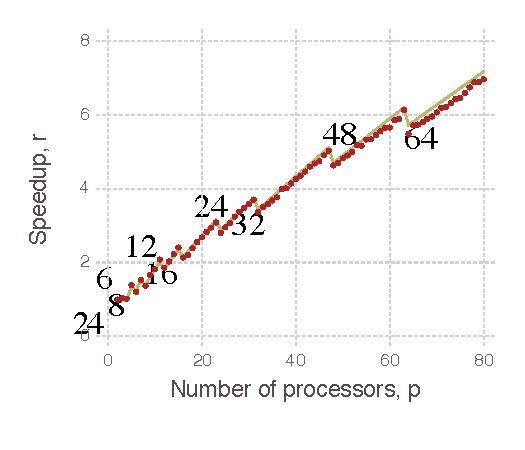
\includegraphics{scaling}
  \caption{Weak scaling of the prefix sum kernels. Speedup ratios are the timings for \code{prefix!} over \code{scanl!}. Plotted also as a solid line is the theoretical speedup ratios $r(p)$ of Eq.~\ref{eq:scaling-theory}.}
  \label{fig:scaling}
\end{figure}

We specifically left out the time needed to broadcast the data to the remote processes, so as to focus only on the execution times of the kernels of interest. We also took care to disable the garbage collector. Julia, like many high-level dynamic languages, provides a garbage collector to aid in memory management. Julia 0.3.1 uses a simple stop-the-world, non-moving, precise mark and sweep garbage collector, where deallocation and finalization of garbage objects may not happen immediately after objects become unused\footnote{The code for Julia's garbage collector may be found at \url{https://github.com/JuliaLang/julia/blob/275afc8b74b9c6ea5d34aefb8085525ff5dfc239/src/gc.c}}~\cite{McCarthy1960}. Therefore, it becomes important to factor out the possible effects of stop-the-world garbage collection. We explicitly disabled garbage collection with \code{gc\_disable()} before running each kernel, then reenabled garbage collection with \code{gc\_enable()} after running each kernel. As an additional precaution, we timed the kernels multiple times and took the minimum time for each kernel so as to reduce fluctuations due to general nondeterministic delays.

\subsection{Operator overloading for visualization}

We can use the code above to use useful computations but we can also visualize its execution!

We make use of the fact that Julia's arrays provide indexing semantics which can be overloaded for custom types~\cite{Bezanson2014}.

We note that code of the form

\begin{minted}{julia}
a[i] = a[j] + a[k]}
\end{minted}
is desugared into syntax of the form

\begin{minted}{julia}
x = getindex(a, j)
y = getindex(a, k)
z = x+y
setindex!(a, z, i)
\end{minted}

There are much more complicated indexing behaviors but we will not touch on them here~\cite{Bezanson2014}.

The nice thing is you can write a custom type that implements \code{getindex} and \code{setindex!}. You don't have to go crazy and implement ALL the indexing semantics of Julia arrays, just the methods that are relevant to your specific application. In this problem all that is really needed is the indexing semantics of a single element.

Now all we have to do is to introduce a custom type that doesn't really do anything but instead records every \code{getindex} and \code{setindex!} operation performed on it. To satisfy the minimum requirements of the prefix reduction algorithm all we need at the moment is for \code{getindex} to return \code{nothing} and to define a dummy method for the associative operator \code{+} that operates on \code{nothing}. \code{nothing} is a value of the special singleton type \code{Void}, akin to Python's \code{none} or Haskell's \code{Nothing}.

Here is a code listing of implementing the trace type

\begin{minted}{julia}
import Base: getindex, setindex!, length

type AccessArray
    length :: Int
    read :: Vector
    history :: Vector
    AccessArray(length)=new(length, {}, {})
end

length(A::AccessArray)=A.length

function getindex(A::AccessArray, i)
    push!(A.read, i)
    nothing
end

function setindex!(A::AccessArray, x, i)
    push!(A.history, (A.read, {i}))
    A.read = {}
end
\end{minted}

\section{Proving correctness}

\cite{Chong2014}
We present our main theoretical result, that
correctness of a generic prefix sum of length n can be established
by showing that the prefix sum is correct for one particular monoid,
the interval of summations monoid, for one particular input.

A monoid is a set together with an associative binary operation which has an identity element in the set. The insight here is that these are exactly the ingredients needed for the parallel prefix algorithm.

In the paper they prove the correctness with respect to something called the interval of summations monoid on one particular input.

With Julia's polymorphism this is pretty trivial to implement!

Monoidal structure has been used to construct a formal algebra of scan algorithms~\cite{Hinze2004}

\section{Related work}

What do other languages do?

Other languages also provide scan primitives like APL~\cite{Iverson1962}, ZPL~\cite{Chamberlain2000}.

MPI provides the \code{MPI\_scan} primitive~\cite{Snir1995,MPI}, and in MPI-2, also the \code{MPI\_Exscan} primitive for exclusive scan.~\cite{MPI2}

Other approaches wish they have genericity, like the Thrust C++ library which uses crazy C++ functors~\cite{Bell2012}.

Does Haskell have something using monoids?

Haskell Accelerate for GPU programming~\cite{Chakravarty2011}. Is it generic? Yes because it works at the code generation level, taking in expressions and emitting longer expressions that compute the prefix sum. In Haskell land these things are criticised for being not statically typed...?

In Julia we use duck typing.

Our approach is rather naive and does not account for the complexities in real world implementations, for example possible synchronicity issues produced by higher levels of the broadcast and reduce trees that could result in bus saturation. In principle this can be handled at the scheduler level in the system but we currently don't have the capabilities to do so in Julia.

\section{Conclusions and outlook}

Here is a way to visualize parallel algorithms and study their correctness. First we show that with pure operator polymorphism we can explicitly show the equivalence of a parallel algorithm and a sequential execution that accomplishes the same computations. This can be used to prove the correctness of a parallel algorithm.

Other variants: e.g. Snir~\cite{Kruskal1985}, Koc~\cite{Egecioglu1992}, doubly pipelined~\cite{Sanders2006}, harmonically scheduled~\cite{Wang1996}, segmented scan~\cite{Sengupta2007}.

Generalization to nonassocative binary operations~\cite{Chen1992}

Visualization is a byproduct of a correct algorithm. This is a powerful new way to understand how algorithms work.

How about something about fast multipole and variants?

\section{Acknowledgments}
We gratefully acknowledge the Julia community, especially Jake Bolewski, for insightful discussions.

Also funding.

\bibliographystyle{abbrv}
\bibliography{prefix}

\appendix

\section{The \code{render} function}
\label{sec:render}

Here are the \code{gate} type and \code{render} function used to generate the figures in Figure~\ref{fig:gates}.

\begin{minted}{julia}
using Compose

type gate
    ins :: Vector
    outs:: Vector
end

function render(G::gate, x, y, y0; ri=0.1, ro=0.25)
    ipoints = [(i, y0+ri) for i in G.ins]
    opoints = [(i, y0+0.5) for i in G.outs]
    igates  = [circle(i..., ri) for i in ipoints]
    ogates  = [circle(i..., ro) for i in opoints]
    lines = [line([i, j]) for i in ipoints,
                              j in opoints]

    compose(context(units=UnitBox(0.5, 0, x, y+1)),
        compose(context(), stroke("black"),
	    fill("white"), igates..., ogates...),
        compose(context(), linewidth(0.3mm),
	    stroke("black"), lines...))
end

function render(A::AccessArray)
    #Scan to find maximum depth
    olast = depth = 0
    for y in A.history
        (any(y[1] .<= olast)) && (depth += 1)
        olast = maximum(y[2])
    end
    maxdepth = depth
    
    olast = depth = 0
    C = {}
    for y in A.history
        (any(y[1] .<= olast)) && (depth += 1)
        push!(C, render(gate(y...), A.length,
	    maxdepth, depth))
        olast = maximum(y[2])
    end
    
    push!(C, compose(context(
      units=UnitBox(0.5, 0, A.length, 1)),
      [line([(i,0), (i,1)]) for i=1:A.length]...,
      linewidth(0.1mm), stroke("grey")))
    compose(context(), C...)
end
\end{minted}

\end{document}
